\section{Results and Discussions}
\label{sec:results}

System outputs were simulated using 4th order Runge-Kutta method on
the state space representation in \eqref{eq:state_space_x}.
Simulation time ranged from $0$s to $6$s with sampling period of $1$ms,
with initial conditions given by \eqref{eq:initial_conditions}:
%
\begin{equation}
    \bm{\theta}_0 = 
    \begin{bmatrix}
        0.5 & 0.1 & 0.05
    \end{bmatrix}^\top,
    \quad
    \dot{\bm{\theta}}_0 = 
    \begin{bmatrix}
        0 & 0 & 0.01
    \end{bmatrix}^\top.
\label{eq:initial_conditions}
\end{equation}

Tremor torque $\bm{\tau}_i$ profiles, presented in \reviewchange{}{Figure} \ref{fig:profiles},
were kept the same in all runs.
The figure also presents the voluntary torques in the deliberate motion scenario, defined as:
\begin{equation}
    \bm{\tau}_v(t) = 
    \begin{bmatrix}
        \sin(2\pi \times 0.1 \times t) \\
        \sin(2\pi \times 0.2 \times t) \\
        \sin(2\pi \times 0.3 \times t) 
    \end{bmatrix}.
\label{eq:tau_v}
\end{equation}
This modeling of voluntary torque compromises between fidelity to real life and ease of implementation. Metrics from 100 simulations with varying physical parameters for $\bm{\tau}_v=\mathbf{0}$ and \eqref{eq:tau_v} are presented in Table \ref{tab:results_averages}. 
%
Figure \ref{fig:plots} shows the effect of EADRC+ZPLP on the uncontrolled system via spectrograms.

\begin{figure}[htbp!]
    \centering
    \caption{
        Tremor torque adopted for all simulations and 
        voluntary torque adopted for deliberate motion scenario.
    }
    \label{fig:profiles}
    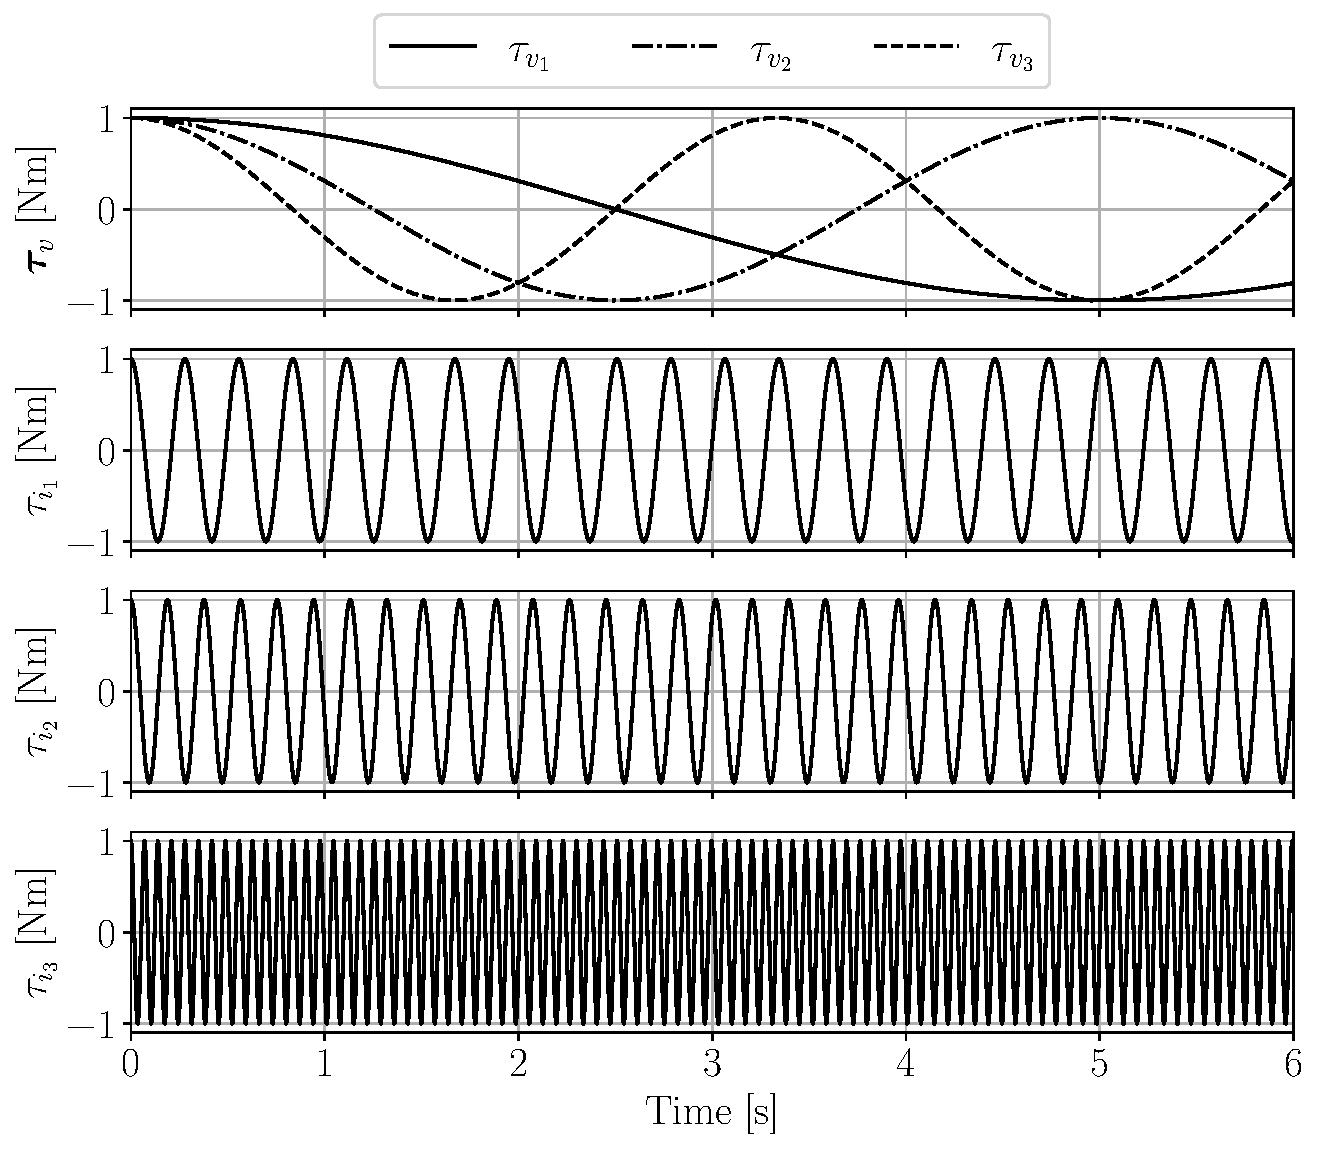
\includegraphics[width=\linewidth]{figures/plots/uncontrolled_amplitude_1.0/torque_profiles_uncontrolled_amplitude_1.0.pdf}
\end{figure}

Simulation results show that EADRC strategies effectively balance tremor attenuation and control effort in a coupled dynamic environment. 
While the DE-PID controller achieved a near-perfect TPSR above 99\%, it serves mainly as an ideal benchmark, relying on full knowledge of voluntary motion and requiring significantly higher actuation. Its TV was about 3.3 times that of EADRC with ZPLP in both scenarios.

\reviewchange{%
\begin{table*}[htbp]
    \centering
    \caption{
        Performance metrics of each control for $\bm\tau_v = \mathbf{0}$.
    }
    \label{tab:results_scenario1}
    \def\arraystretch{1.3}
    \begin{tabular}{
    c | c | c | c | c | c | c 
}
    \multirow{2}{*}{Controller} &
    \multicolumn{4}{c}{Response Signal} &
    \multicolumn{2}{|c}{Control Signal} \\
    \cline{2-7}
    &
    TPSR [\%] & 
    % ASR [\%] & 
    $R^2$ & 
    Entropy [bits] & 
    IAE [rad$\times$s] & 
    % ISE & 
    % ITAE & 
    % ITSE & 
    Power [(N$\times$m)$^2$] & 
    TV [N$\times$m$\times$s] 
    % IAC & 
    % ISC
\\
    \hline
%AFE & -150.62 $\pm$ 238.34 & -2.53 $\pm$ 1.94 & 5.36 $\pm$ 0.26 & 1.74 $\pm$ 0.45 & 0.76 $\pm$ 0.41 & 247.08 $\pm$ 71.96 \\
EADRC+EBMFLC & 40.67 $\pm$ 64.69 & 0.41 $\pm$ 0.14 & 5.19 $\pm$ 0.15 & 0.82 $\pm$ 0.26 & 0.49 $\pm$ 0.25 & 301.32 $\pm$ 83.25 \\
EADRC+ZPLP & 52.47 $\pm$ 46.16 & 0.44 $\pm$ 0.18 & 5.18 $\pm$ 0.17 & 0.73 $\pm$ 0.18 & 0.32 $\pm$ 0.12 & 255.43 $\pm$ 47.00 \\
%Gallego-PI & -147.98 $\pm$ 592.27 & -1.29 $\pm$ 2.18 & 5.08 $\pm$ 0.32 & 1.51 $\pm$ 1.10 & 2.21 $\pm$ 11.28 & 135.53 $\pm$ 46.99 \\
DE-PID & 99.90 $\pm$ 0.10 & 1.00 $\pm$ 0.00 & 4.85 $\pm$ 0.11 & 0.03 $\pm$ 0.01 & 0.88 $\pm$ 0.33 & 408.58 $\pm$ 8.93 \\
IMC-PID & -37.55 $\pm$ 279.40 & -0.16 $\pm$ 0.42 & 5.48 $\pm$ 0.14 & 1.13 $\pm$ 0.52 & 0.37 $\pm$ 0.23 & 183.32 $\pm$ 24.05 \\
\end{tabular}

\end{table*}
%
\begin{table*}[htbp]
    \centering
    \caption{
        Performance metrics of each control for $\bm\tau_v$ given by \eqref{eq:tau_v}.
    }
    \label{tab:results_scenario2}
    \def\arraystretch{1.3}
    \begin{tabular}{
    c | c | c | c | c | c | c 
}
    \multirow{2}{*}{Controller} &
    \multicolumn{4}{c}{Response Signal} &
    \multicolumn{2}{|c}{Control Signal} \\
    \cline{2-7}
    &
    TPSR [\%] & 
    % ASR [\%] & 
    $R^2$ & 
    Entropy [bits] & 
    IAE [rad$\times$s] & 
    % ISE & 
    % ITAE & 
    % ITSE & 
    Power [(N$\times$m)$^2$] & 
    TV [N$\times$m$\times$s] 
    % IAC & 
    % ISC
\\
    \hline
%AFE & -139.58 $\pm$ 315.12 & -1.63 $\pm$ 1.44 & 5.28 $\pm$ 0.25 & 1.72 $\pm$ 0.43 & 0.76 $\pm$ 0.35 & 229.81 $\pm$ 70.26 \\
EADRC+EBMFLC & 49.78 $\pm$ 51.24 & 0.46 $\pm$ 0.11 & 5.24 $\pm$ 0.13 & 0.82 $\pm$ 0.25 & 0.50 $\pm$ 0.24 & 301.84 $\pm$ 81.80 \\
EADRC+ZPLP & 61.31 $\pm$ 33.58 & 0.48 $\pm$ 0.16 & 5.24 $\pm$ 0.13 & 0.74 $\pm$ 0.18 & 0.33 $\pm$ 0.11 & 258.39 $\pm$ 43.92 \\
%Gallego-PI & -42.61 $\pm$ 132.60 & -0.66 $\pm$ 0.63 & 5.13 $\pm$ 0.24 & 1.38 $\pm$ 0.40 & 0.75 $\pm$ 1.15 & 124.11 $\pm$ 24.17 \\
DE-PID & 99.92 $\pm$ 0.08 & 1.00 $\pm$ 0.00 & 4.93 $\pm$ 0.10 & 0.03 $\pm$ 0.01 & 0.90 $\pm$ 0.34 & 409.52 $\pm$ 8.96 \\
IMC-PID & 4.79 $\pm$ 115.92 & -0.05 $\pm$ 0.33 & 5.48 $\pm$ 0.13 & 1.12 $\pm$ 0.45 & 0.40 $\pm$ 0.20 & 192.98 $\pm$ 20.43 \\
\end{tabular}

\end{table*}
}{%
    \begin{table*}[htbp]
        \centering
        \caption{
            Average performance metrics of each control strategy.
        }
        \label{tab:results_averages}
        \def\arraystretch{1.3}
        \begin{tabular}{
    c | c | c | c | c | c | c | c 
}
    &
    \multirow{2}{*}{Controller} &
    \multicolumn{4}{c}{Response Signal} &
    \multicolumn{2}{|c}{Control Signal} \\
    \cline{3-8}
    &&
    TPSR [\%] & 
    $R^2$ & 
    Entropy [bits] & 
    IAE [rad$\times$s] & 
    Power [(N$\times$m)$^2$] & 
    TV [N$\times$m$\times$s] 
\\
    \hline
    \multirow{4}{*}{\rotatebox{90}{$\bm{\tau}_v=\mathbf{0}$}}
    &
EADRC+EBMFLC & 40.67 $\pm$ 64.69 & 0.41 $\pm$ 0.14 & 5.19 $\pm$ 0.15 & 0.82 $\pm$ 0.26 & 0.49 $\pm$ 0.25 & 301.32 $\pm$ 83.25 \\ &
EADRC+ZPLP & 52.47 $\pm$ 46.16 & 0.44 $\pm$ 0.18 & 5.18 $\pm$ 0.17 & 0.73 $\pm$ 0.18 & 0.32 $\pm$ 0.12 & 255.43 $\pm$ 47.00 \\ &
DE-PID & 99.90 $\pm$ 0.10 & 1.00 $\pm$ 0.00 & 4.85 $\pm$ 0.11 & 0.03 $\pm$ 0.01 & 0.88 $\pm$ 0.33 & 408.58 $\pm$ 8.93 \\ &
IMC-PID & -37.55 $\pm$ 279.40 & -0.16 $\pm$ 0.42 & 5.48 $\pm$ 0.14 & 1.13 $\pm$ 0.52 & 0.37 $\pm$ 0.23 & 183.32 $\pm$ 24.05 
\\
    \hline
    \multirow{4}{*}{\rotatebox{90}{\tiny $\bm{\tau}_v$ as in \eqref{eq:tau_v}}}
    &
EADRC+EBMFLC & 49.78 $\pm$ 51.24 & 0.46 $\pm$ 0.11 & 5.24 $\pm$ 0.13 & 0.82 $\pm$ 0.25 & 0.50 $\pm$ 0.24 & 301.84 $\pm$ 81.80 \\ &
EADRC+ZPLP & 61.31 $\pm$ 33.58 & 0.48 $\pm$ 0.16 & 5.24 $\pm$ 0.13 & 0.74 $\pm$ 0.18 & 0.33 $\pm$ 0.11 & 258.39 $\pm$ 43.92 \\ &
%Gallego-PI & -42.61 $\pm$ 132.60 & -0.66 $\pm$ 0.63 & 5.13 $\pm$ 0.24 & 1.38 $\pm$ 0.40 & 0.75 $\pm$ 1.15 & 124.11 $\pm$ 24.17 \\
DE-PID & 99.92 $\pm$ 0.08 & 1.00 $\pm$ 0.00 & 4.93 $\pm$ 0.10 & 0.03 $\pm$ 0.01 & 0.90 $\pm$ 0.34 & 409.52 $\pm$ 8.96 \\ &
IMC-PID & 4.79 $\pm$ 115.92 & -0.05 $\pm$ 0.33 & 5.48 $\pm$ 0.13 & 1.12 $\pm$ 0.45 & 0.40 $\pm$ 0.20 & 192.98 $\pm$ 20.43 \\
\end{tabular}

    \end{table*}
}

\reviewchange{%
    In contrast, IMC-PID and Gallego-PI exhibited much lower TPSR, indicating sensitivity to coupled perturbations in a 3-DoF model.
}{% 
    To substantiate these comparisons statistically, a paired Wilcoxon signed-rank test was applied per metric and scenario, comparing EADRC+ZPLP against each baseline controller across the same 100 Monte Carlo parameter draws. 
    
    According to Table \ref{tab:wilcoxon}, in both scenarios EADRC+ZPLP outperforms EADRC+EBMFLC on every metric but Entropy ($p < 0.001$): 
    it achieves higher tremor suppression (TPSR, $r \geq 0.56$; IAE, $r \leq -0.68$) 
    while requiring less control effort (TV, $r \leq -0.81$), with lower control Power in every one of the 100 paired trials ($r = -1.00$), 
    supporting the claimed balance between attenuation and actuation. 
    Entropy did not differ significantly in the resting scenario ($p = 0.73$) and was moderately lower for EADRC+ZPLP in the moving one ($r = -0.32$). 
    
    Differences against DE-PID were significant for every metric in both scenarios with maximal or near-maximal effect size 
    ($|r| \geq 0.99$), reflecting that DE-PID suppressed tremor better than EADRC+ZPLP in practically every one of the 100 paired trials, 
    at the cost of higher control effort in all of them.
    %
    This is consistent with its role as an idealized upper-bound benchmark rather than a practical competitor.
    
    EADRC+ZPLP suppressed tremor better than IMC-PID in nearly every paired trial ($|r| \geq 0.94$ for TPSR, $R^2$ and IAE) 
    while requiring less control effort in every one of them (Power and TV, $r = -1.00$). 
    IMC-PID, tuned on the uncoupled nominal wrist, showed growing oscillations in 4 (resting) and 5 (moving) of the 99 perturbed models, 
    which explains its negative average TPSR despite median values above 50\%.
}

\reviewchange{}{
\begin{table}[htb]
    \centering
    \caption{% 
        Holm-Bonferroni corrected $p$-value and rank-biserial correlation $r$ 
        for paired Wilcoxon signed-rank tests.
    }
    \label{tab:wilcoxon}
    \resizebox{\linewidth}{!}{%
        \def\arraystretch{1.3}
        \begin{tabular}{c | c | cc | cc | cc}
    & \multirow{3}{*}{Metric} 
    & \multicolumn{6}{c}{EADRC+ZPLP vs. $\cdots$}
\\
\cline{3-8}
    &
    & \multicolumn{2}{c}{EADRC+EBMFLC} 
    & \multicolumn{2}{c}{DE-PID} 
    & \multicolumn{2}{c}{IMC-PID} \\
\cline{3-8}
    &
    & $p$ & $r$
    & $p$ & $r$
    & $p$ & $r$ \\
\hline
    \multirow{6}{*}{\rotatebox{90}{$\bm{\tau}_v = \mathbf{0}$}} & TPSR [\%] & 1.000 & -0.00 & $<$0.001 & -1.00 & $<$0.001 & +0.73 \\
    & $R^2$ & $<$0.001 & +0.53 & $<$0.001 & -1.00 & $<$0.001 & +0.97 \\
    & Entropy [bits] & $<$0.001 & -0.44 & $<$0.001 & +0.96 & $<$0.001 & -0.95 \\
    & IAE [rad$\times$s] & 1.000 & -0.03 & $<$0.001 & +1.00 & $<$0.001 & -0.81 \\
    & Power [(N$\times$m)$^2$] & 0.001 & -0.43 & $<$0.001 & -1.00 & 0.665 & -0.14 \\
    & TV [N$\times$m$\times$s] & 0.018 & -0.33 & $<$0.001 & -1.00 & $<$0.001 & +0.95 \\
\hline
    \multirow{6}{*}{\rotatebox{90}{$\bm{\tau}_v$ as in \eqref{eq:tau_v}}} & TPSR [\%] & 1.000 & +0.09 & $<$0.001 & -1.00 & $<$0.001 & +0.71 \\
    & $R^2$ & 0.039 & +0.31 & $<$0.001 & -1.00 & $<$0.001 & +0.99 \\
    & Entropy [bits] & 0.144 & -0.24 & $<$0.001 & +0.97 & $<$0.001 & -0.96 \\
    & IAE [rad$\times$s] & 1.000 & -0.08 & $<$0.001 & +1.00 & $<$0.001 & -0.76 \\
    & Power [(N$\times$m)$^2$] & $<$0.001 & -0.44 & $<$0.001 & -1.00 & 1.000 & -0.09 \\
    & TV [N$\times$m$\times$s] & 0.034 & -0.32 & $<$0.001 & -1.00 & $<$0.001 & +0.97 \\
\end{tabular}%
    }
\end{table}
}

While EADRC+ZPLP has been successful in suppressing tremor regardless of the voluntary motion estimator employed,
it demonstrated somewhat poor capacity in mitigating lower-frequency tremors, 
as spectrograms in Figure \ref{fig:plots} show.
%
This could indicate that the filtering process in voluntary motion estimation was not sufficient,
and EADRC did not factor unmitigated tremor as part of the total disturbance.

\begin{figure}[htb]
    \centering
    \captionof{figure}{Spectrograms of the uncompensated and compensated tremor of both scenarios.}
    \label{fig:plots}
    \begin{subfigure}{.685\linewidth}
        \centering
        \caption{Uncompensated resting tremor}
        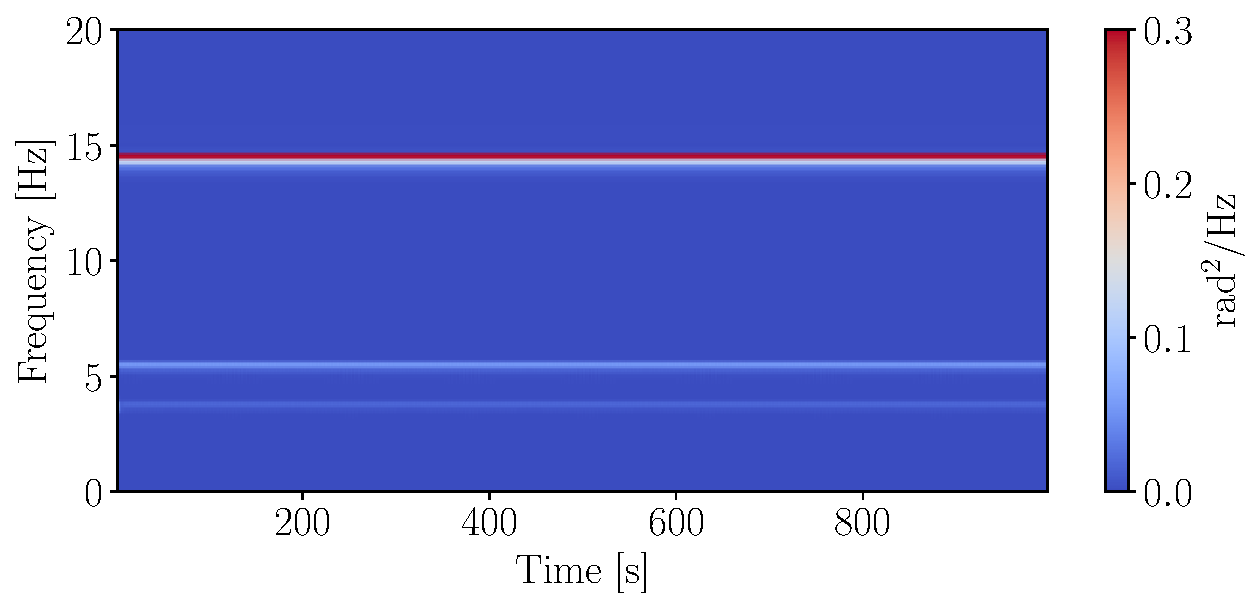
\includegraphics[width=\linewidth]{figures/plots/uncontrolled_amplitude_0.0/spectrogram_response_uncontrolled_amplitude_0.0.pdf}
    \end{subfigure}
    %
    \begin{subfigure}{.685\linewidth}
        \centering
        \caption{Compensated resting tremor}
        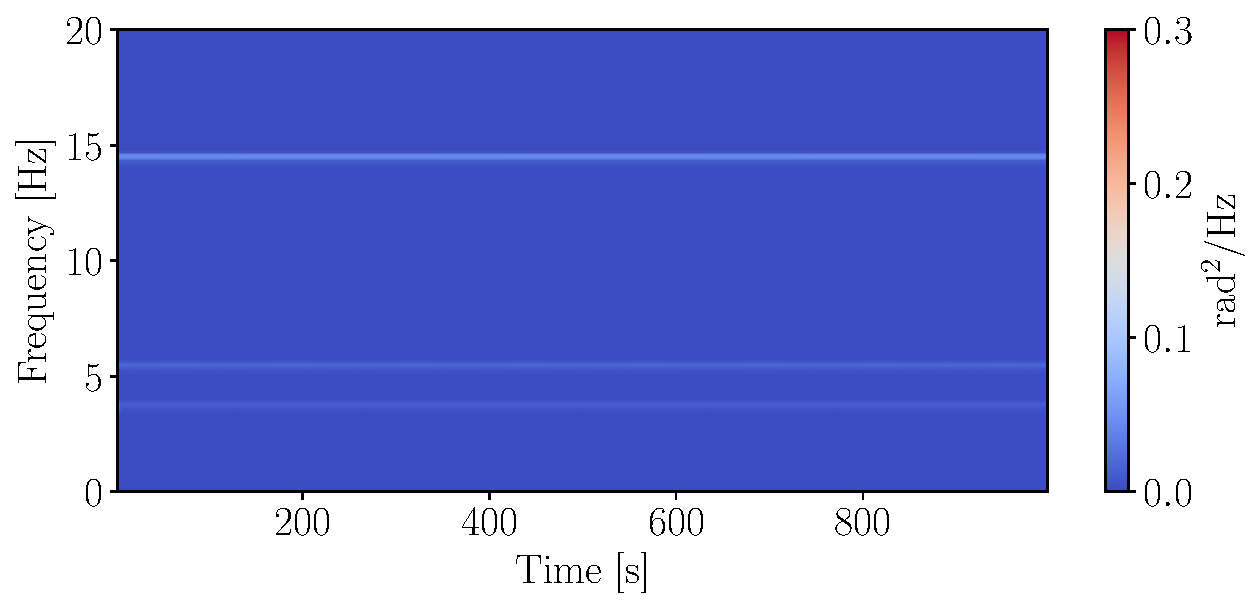
\includegraphics[width=\linewidth]{figures/plots/eadrc_ebmflc_amplitude_0.0/spectrogram_response_eadrc_ebmflc_amplitude_0.0.pdf}
    \end{subfigure}
    %
    \begin{subfigure}{.685\linewidth}
        \centering
        \caption{Uncompensated moving tremor}
        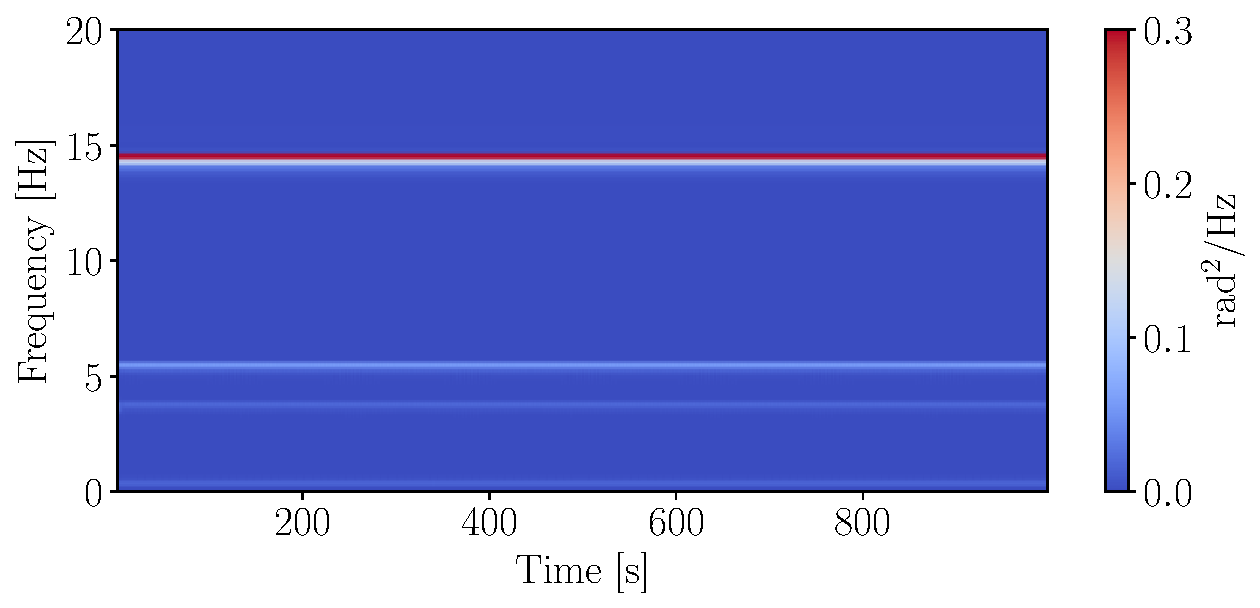
\includegraphics[width=\linewidth]{figures/plots/uncontrolled_amplitude_1.0/spectrogram_response_uncontrolled_amplitude_1.0.pdf}
    \end{subfigure}
    %
    \begin{subfigure}{.685\linewidth}
        \centering
        \caption{Compensated moving tremor}
        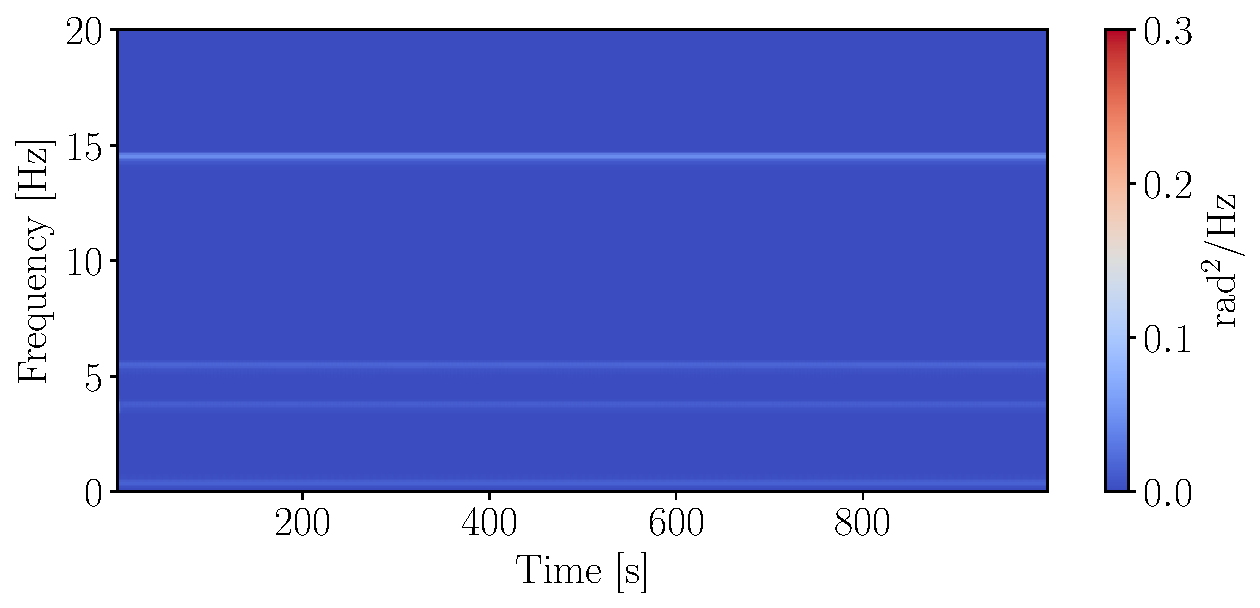
\includegraphics[width=\linewidth]{figures/plots/eadrc_ebmflc_amplitude_1.0/spectrogram_response_eadrc_ebmflc_amplitude_1.0.pdf}
    \end{subfigure}
\end{figure}